\section{Simulation study}\label{sec:simulation}

All data in this section are synthetic. Every dataset is simulated from a model whose
parameters we chose, so the truth is known. No real incident data are used, and nothing in
this section is a finding about antisemitic incidents. Every number is taken from
\texttt{results/sim\_results.json}, which \texttt{code/run\_experiments.py} writes; the
design table, configurations, seeds, software versions, run times and code hashes are in
\cref{app:simdetails}. Time is measured in arbitrary units, which we call days.

\subsection{Design}\label{sec:sim-design}

Six experiments test the claims of
\cref{sec:identification,sec:attribution,sec:estimation,sec:forecasting}
(\cref{tab:sim-design}): recovery by EM (E1), surge attribution (E5), spurious contagion
(E2), thinning (E3), the online-to-offline test (E4) and alerting (E6). Data are drawn by
exact cluster simulation (\cref{app:comp-sim}) from the empty history at time $0$, with
exponential kernels and shock responses. Fits use \cref{alg:em} with the exact window
terms, one decay rate $\beta$ for all excitation kernels, one response rate $\eta$ for all
streams unless stated otherwise, the default multistart over decay rates and a relative
tolerance of $10^{-8}$ ($10^{-9}$ in E4). Intervals are nominal $95\%$ Wald intervals from the
observed information (\cref{app:comp-se}), delta-method for derived quantities. Monte Carlo
standard errors (MC SE) are in parentheses (\cref{app:sim-mcse}); for a coverage of $0.95$
it is $0.022$ with $R=100$ replicates and $0.034$ with $R=40$.

\subsection{E1 and E5: recovery and attribution}\label{sec:sim-recovery}\label{sec:sim-attribution}

E1 checks EM on the shock-augmented model, whose calendar of events breaks the
stationarity assumed in \cref{sec:est-mle}; E5 checks the closed forms of
\cref{thm:attribution,prop:irf} and the ancestral reading of the online channel
(\cref{prop:at-channel}(a)) against branching labels. \Cref{app:sim-e1e5} gives the
design and full results. In E1 ($M=3$, $\spr(\Amat)=0.485$,
$R=100$ per $T$) all 200 fits converged with positive definite information. At $T=2000$ the
nine $\alpha_{kj}$ have mean $|$bias$|$ $0.002$, mean RMSE $0.026$ and coverage
$0.92$--$0.99$, as do the entries of the multiplier $\Mmat=(\Imat-\Amat)^{-1}$; doubling $T$
reduces the RMSE by about $2^{-1/2}$. The online loading $\upsilon_3=6$ is overestimated by
$0.137$ ($0.079$), with the same sign at $T=1000$. The design is benign: $\spr(\Amat)$ is far
from one and every $\alpha_{kj}$ far from zero. In E5 the exact decomposition agrees with
the branching labels of 20{,}000 paths: over 11 quantities per horizon the largest $|z|$
is $1.50$, and the online-channel contagion of offline region A at $H=14$ is $5.779$
exactly and $5.800$ ($0.026$) by simulation. Plug-in estimates from the E1 fits cover in
$0.91$--$0.96$ of replicates over 45 attribution quantities at $T=2000$
(\cref{tab:sim-e4e5}(b) in \cref{app:sim-e1e5}). The direct component is less precise than the contagion component
(RMSE $1.598$ against $1.153$ for region A): the loadings rest on 17 events, the branching
matrix on thousands of incidents.

\subsection{E2: spurious contagion}\label{sec:sim-spurious}

\paragraph{Claim} Without contagion but with a fluctuating rate, a constant-background
Hawkes fit finds contagion. For second-order estimators the pseudo-true branching ratio is
$n^*=1-(1+\kappa)^{-1/2}$ (\cref{thm:spurious}(a)--(c)); for maximum likelihood,
\cref{thm:spurious}(d) proves only that it is positive, and \cref{rem:th-spurious}(ii)
leaves its relation to $n^*$ open. Known shock times restore identification
(\cref{cor:equiv-id}(i)); we also ask whether a flexible background does.

\paragraph{Design} Every dataset has mean rate $\Lambda=2$ and no contagion. Two families
are shot-noise Cox processes (\cref{def:th-sncox}) with shock decay $\gamma=0.5$ and $m$
incidents per shock: \emph{rare} ($m=16$, $\kappa\in\{0.5,1,2,4,8\}$) and \emph{frequent}
($m=4$, $\kappa\in\{0.5,1,2,3\}$). The third family switches the rate between
$\Lambda\pm\delta$ at rate $0.01$ in each direction, with $\kappa\in\{0.5,2,8\}$. With
$T=1000$ and $R=20$, rare-family paths carry $1$--$77$ shocks (including a 40-day lead-in)
and frequent-family paths $54$--$424$ (\cref{tab:sim-e2e3}(a)), so a difference between the
families could be finite-sample bias. To separate the two, the rare family at
$\kappa\in\{2,4\}$ was also run with $T=10{,}000$ ($135$--$341$ shocks per path; constant
background only). We fit (i) a constant background; (ii) a log-linear cubic
B-spline background with 20 basis functions, knots about 59 days apart; and (iii) a constant
background with the shock times as a calendar ($S_e=1$; loading and response rate
estimated), for all rare configurations and the frequent ones with $\kappa\le1$
(\cref{app:sim-config} explains the cost of the others). For the shot-noise families we also
compute the dispersion functional $n_F=1-F^{-1/2}$ of \cref{thm:spurious}(c) from counts in
25-day bins; its finite-window target is $n^*_w$ (\cref{app:sim-config}).

\paragraph{What is reported} Without contagion the likelihood has a ridge on which the decay
tends to zero while $\hat\alpha$ grows and the in-window offspring stay few. Flagging a fit
as on the ridge when $\hat\beta T<1$ (its kernel has not decayed within the window), nine
of the 620 fits at $T=1000$ are on it: six of the 140 shocks-known fits, two
constant-background fits and one spline fit for slow switching (\cref{tab:sim-e2e3}(a)).
Eight have $\hat\beta T<0.1$ and $\hat\alpha$ between $1.7$ and $29.1$; no long-window fit
is on the ridge. We therefore report the in-window branching ratio
$\hat n_{\mathrm{eff}}=\hat\alpha\,N(T)^{-1}\sum_l\{1-e^{-\hat\beta(T-t_l)}\}$, the expected
number of in-window offspring per incident and the share of incidents that EM attributes to
self-excitation. For the constant-background fits to the shot-noise families it equals
$\hat\alpha$ to within $0.003$. Its distribution is skewed near zero, so
\cref{tab:sim-e2e3}(a) gives medians with the means: the mean spline estimate for slow
switching at $\kappa=8$, for example, is $0.028$, but $0.018$ without its ridge fit, and the
median is $0.003$.

\paragraph{Constant background} Spurious contagion appears in every configuration and grows
with $\kappa$ (\cref{fig:sim-spurious}(a)). For the rare family the gaps
$\hat n_{\mathrm{eff}}-n^*$ are $-0.059$ ($0.021$), $-0.018$ ($0.017$), $-0.058$ ($0.014$),
$-0.066$ ($0.0085$) and $-0.039$ ($0.008$) for $\kappa=0.5,1,2,4,8$; for the frequent family
they lie within $\pm0.009$, each within one MC SE. The rare-family gaps are not
finite-sample bias. With $T=10{,}000$ they are $-0.062$ ($0.004$) at $\kappa=2$ and $-0.068$
($0.002$) at $\kappa=4$, as large as at $T=1000$, although the long paths carry as many
shocks as the frequent-family paths. Over the same tenfold increase in $T$ the dispersion
estimator settles on its target ($0.408$ and $0.541$, MC SE $0.006$ and $0.004$, against
$n^*_w=0.407$ and $0.538$). The maximum likelihood estimator thus converges to a pseudo-true
value below $n^*$ when shocks are rare and large, as \cref{rem:th-spurious}(ii) allows: the
likelihood responds to structure beyond second order, where the members of the matched
family of \cref{thm:equiv} differ. For slow switching the fits fall far short of $n^*$
($0.069$, $0.216$ and $0.435$ against $0.184$, $0.423$ and $0.667$); with about ten regime
switches in 1000 days, a finite-window effect remains a second explanation there, which we
did not test.

\paragraph{Remedies} A spline background removes the artefact of slow switching (means
$0.008$, $0.007$ and $0.028$; medians $0.005$, $0.002$ and $0.003$) but not that of fast
shocks (\cref{fig:sim-spurious}(b)): it lowers $\hat n_{\mathrm{eff}}$ by only
$0.05$--$0.10$, for example from $0.628$ to $0.581$ for the rare family at $\kappa=8$.
Responses that decay within days cannot be represented by knots two months apart
(\cref{sec:est-mle}); a background flexible enough to follow them would also absorb genuine
contagion, which E2 does not measure. Known shock times largely remove the artefact, where
tested: for the rare family at every $\kappa$ and the frequent family at $\kappa\le1$,
$\hat n_{\mathrm{eff}}$ has means $0.035$--$0.076$ (medians $0.012$--$0.055$) against
$0.12$--$0.63$ without the calendar, and the loadings are recovered ($15.2$--$16.4$ against
$m=16$; $3.94$ and $3.87$ against $m=4$). The small positive remainder is expected of an
estimator constrained to $\alpha\ge0$ at a true value on the boundary (\cref{prop:lrt}(b)).
Where tested, the conclusion is that of \cref{cor:equiv-id}(i): spurious contagion from
unrecorded shocks is removed by recording the shocks, not by smoothing.

\begin{table}[tbp]
\centering
\caption{Results of E2 and E3 (synthetic data). (a) E2, data \emph{without} contagion:
in-window branching ratio $\hat n_{\mathrm{eff}}$, mean (median) over $R=20$ replicates;
shocks per path, median [minimum, maximum], including the 40-day lead-in; Ridge: number of
fits with $\hat\beta T<1$ among the constant, spline and shocks-known fits (a hyphen: fit
not run).
(b) E3 at $p=0.4$: naive and corrected estimates of $n$ ($R=40$). Floor: the $p$-term
$r\,n(1-n)(2-n)/2$ of the standard deviation in \eqref{eq:th-delta}, for relative error $r$
of $\hat p$. Cov.: coverage of nominal $95\%$ intervals.}
\label{tab:sim-e2e3}
\footnotesize
\setlength{\tabcolsep}{4.2pt}
\renewcommand{\arraystretch}{1.0}
\textit{(a) E2: spurious contagion}\par\smallskip
% Generated by code/make_figures.py from results/sim_results.json -- do not edit by hand.
% E2 (no contagion). n_eff = alpha_hat * mean(1 - exp(-beta_hat (T - t_l))): mean (median) over replicates.
% Shocks: shocks per path, median [min, max] (incl. the 40-day lead-in). Ridge: fits with beta_hat * T < 1,
% for the constant / spline / shocks-known fits ('-' = fit not run).
\begin{tabular}{@{}lrrcrcccc@{}}
\toprule
 & & & & & \multicolumn{3}{c}{$\hat n_{\mathrm{eff}}$, mean (median)} & \\
\cmidrule(lr){6-8}
Family & $\kappa$ & $T$ & Shocks per path & $n^*$ & Constant & Spline & Shocks known & Ridge \\
\midrule
Rare ($m=16$) & 0.5 & 1000 & 3.5 [1, 8] & 0.184 & 0.124 (0.119) & 0.064 (0.053) & 0.035 (0.023) & 0/0/0 \\
 & 1 & 1000 & 9 [4, 20] & 0.293 & 0.275 (0.294) & 0.174 (0.192) & 0.055 (0.055) & 0/0/1 \\
 & 2 & 1000 & 15.5 [9, 30] & 0.423 & 0.365 (0.392) & 0.288 (0.299) & 0.048 (0.017) & 0/0/2 \\
 & 4 & 1000 & 34.5 [25, 43] & 0.553 & 0.487 (0.483) & 0.430 (0.436) & 0.041 (0.033) & 0/0/0 \\
 & 8 & 1000 & 65.5 [52, 77] & 0.667 & 0.628 (0.628) & 0.581 (0.582) & 0.044 (0.023) & 0/0/0 \\
\addlinespace
Frequent ($m=4$) & 0.5 & 1000 & 69.5 [54, 86] & 0.184 & 0.181 (0.174) & 0.088 (0.085) & 0.047 (0.012) & 0/0/1 \\
 & 1 & 1000 & 133.5 [104, 149] & 0.293 & 0.284 (0.292) & 0.188 (0.181) & 0.076 (0.048) & 0/0/2 \\
 & 2 & 1000 & 258 [240, 290] & 0.423 & 0.431 (0.426) & 0.355 (0.347) & --- & 0/0/- \\
 & 3 & 1000 & 390 [349, 424] & 0.500 & 0.497 (0.494) & 0.438 (0.434) & --- & 0/0/- \\
\addlinespace
Slow switching & 0.5 & 1000 & --- & 0.184 & 0.069 (0.066) & 0.008 (0.005) & --- & 0/0/- \\
 & 2 & 1000 & --- & 0.423 & 0.216 (0.221) & 0.007 (0.002) & --- & 2/0/- \\
 & 8 & 1000 & --- & 0.667 & 0.435 (0.425) & 0.028 (0.003) & --- & 0/1/- \\
\addlinespace
Rare ($m=16$), long & 2 & 10000 & 157.5 [135, 183] & 0.423 & 0.361 (0.359) & --- & --- & 0/-/- \\
 & 4 & 10000 & 322 [293, 341] & 0.553 & 0.484 (0.483) & --- & --- & 0/-/- \\
\bottomrule
\end{tabular}

\par\bigskip
\textit{(b) E3: thinning and the dark-figure correction}\par\smallskip
% Generated by code/make_figures.py from results/sim_results.json -- do not edit by hand.
% E3 at p = 0.4. Floor: r n (1 - n)(2 - n) / 2, the p-term of eq:th-delta for relative error r of p_hat.
% Cov.: coverage (%) of nominal 95% intervals (R = 40).
\begin{tabular}{@{}llrrrrrr@{}}
\toprule
Setting & Estimator & Target & Mean & Bias & RMSE & Floor & Cov.\ (\%) \\
\midrule
$n=0.5$, $p=0.4$ & $\hat n'$ (naive) & 0.500 & 0.315 & $-$0.185 & 0.189 & --- & 2.5 \\
 & $h_p^{-1}(\hat n')$, $p$ known & 0.500 & 0.488 & $-$0.012 & 0.042 & --- & 95.0 \\
 & $h_{\hat p}^{-1}(\hat n')$, $10\%$ error & 0.500 & 0.491 & $-$0.009 & 0.046 & 0.019 & 97.5 \\
 & $h_{\hat p}^{-1}(\hat n')$, $30\%$ error & 0.500 & 0.503 & $+$0.003 & 0.073 & 0.056 & 87.5 \\
 & $h_{\hat p}^{-1}(\hat n')$, $50\%$ error & 0.500 & 0.525 & $+$0.025 & 0.128 & 0.094 & 85.0 \\
\addlinespace
$n=0.7$, $p=0.4$ & $\hat n'$ (naive) & 0.700 & 0.553 & $-$0.147 & 0.152 & --- & 5.0 \\
 & $h_p^{-1}(\hat n')$, $p$ known & 0.700 & 0.698 & $-$0.002 & 0.031 & --- & 95.0 \\
 & $h_{\hat p}^{-1}(\hat n')$, $10\%$ error & 0.700 & 0.704 & $+$0.004 & 0.035 & 0.014 & 92.5 \\
 & $h_{\hat p}^{-1}(\hat n')$, $30\%$ error & 0.700 & 0.720 & $+$0.020 & 0.061 & 0.041 & 80.0 \\
 & $h_{\hat p}^{-1}(\hat n')$, $50\%$ error & 0.700 & 0.742 & $+$0.042 & 0.101 & 0.068 & 80.0 \\
\addlinespace
heterog., $\mathrm{Cov}(p_X,n_X)>0$ & $h_{\bar p}^{-1}(\hat n'')$ & 0.500 & 0.567 & $+$0.067 & 0.076 & --- & --- \\
\bottomrule
\end{tabular}

\end{table}

\begin{figure}[tbp]
\centering
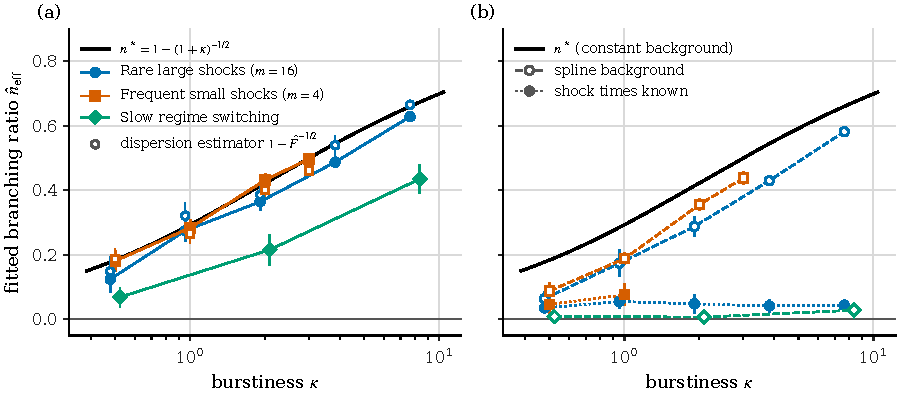
\includegraphics[width=6.0in]{figures/fig-sim-spurious.pdf}
\caption{E2, spurious contagion in synthetic data with \emph{no} contagion ($R=20$ per
point; bars $\pm1.96$ MC SE). (a) $\hat n_{\mathrm{eff}}$ of constant-background fits
against the burstiness $\kappa$ ($T=1000$), with $n^*$ (line), the dispersion estimator
(open markers) and the rare family with $T=10{,}000$ (stars, shifted right). (b) Spline
background (open markers, dashed) and shock times known (filled markers, dotted). Means;
medians are in \cref{tab:sim-e2e3}(a).}
\label{fig:sim-spurious}
\end{figure}

\subsection{E3: thinning and the dark-figure correction}\label{sec:sim-thinning}

\paragraph{Claim} Independent recording with probability $p$ maps $n$ to $n'=h_p(n)$
(\cref{thm:thinning}), and $h_p^{-1}$ undoes the attenuation (\cref{cor:th-darkfig}), with a
floor on its precision set by the uncertainty about $p$. \Cref{thm:thinning}(d) leaves open
whether the maximum likelihood estimator converges to $n'$. Under heterogeneous recording
the homogeneous correction errs as \cref{prop:th-hetthin} predicts.

\paragraph{Design} A univariate exponential Hawkes process with $\beta=1$, $\Lambda=2$,
$T=1500$ and $n\in\{0.3,0.5,0.7\}$ ($R=40$) is thinned at $p\in\{1,0.8,0.6,0.4,0.2\}$, with
nested recorded sets, and refitted. The \emph{naive} estimate is $\hat n'$; the
\emph{corrected} estimate is $h_p^{-1}(\hat n')$ with the delta-method variance
\eqref{eq:th-delta}, with $p$ known or estimated by $\hat p=p(1+rZ)$, $Z\sim N(0,1)$,
clipped to $[0.02,1]$, with standard error $r\hat p$ and relative error
$r\in\{10,30,50\}\%$ (one $Z$ for all three). In the heterogeneous design two equally likely
marks have $n_x=(0.1,0.9)$, so $\bar n=0.5$, and are recorded with
$(p_1,p_2)\in\{(0.2,0.8),(0.5,0.5),(0.8,0.2),(1,1)\}$ ($R=30$).

\paragraph{Results} The maximum likelihood estimate tracks $n'(p)$: over the 15
combinations of $n$ and $p$, $|\text{mean of }\hat n'-n'(p)|\le0.0104$ (MC SE $0.0062$).
Ignoring thinning is not harmless: at $n=0.5$ the naive interval covers the true $n$ in
$0.975$, $0.825$, $0.175$, $0.025$ and $0$ of replicates for $p=1,\dots,0.2$
(\cref{fig:sim-thinning}(a)). The correction with $p$ known has bias between $-0.0004$ and
$-0.0155$ and coverage $0.925$--$1$ at $n=0.5$ and $0.90$--$0.95$ at $n=0.7$, and $10\%$
error in $\hat p$ changes little (\cref{tab:sim-e2e3}(b)). The exception is weak excitation
with heavy thinning: at $n=0.3$ and $p\le0.4$, $n'$ is within a few standard errors of the
boundary (\cref{prop:lrt}(b)), the fitted decay is erratic (means $23.4$ and $110.8$ against
$0.83$ and $0.77$) and coverage falls to $0.85$ and $0.70$; profile-likelihood or bootstrap
intervals are needed there.

Larger errors in $\hat p$ expose the floor of \cref{cor:th-darkfig}. With
$\mathrm{SD}(\hat p)=rp$, the second term of \eqref{eq:th-delta} contributes the standard
deviation $r\,n(1-n)(2-n)/2$, which depends on neither $p$ nor $T$; at $n=0.5$ it is $0.019$,
$0.056$ and $0.094$ for $r=10$, $30$ and $50\%$. Across the five values of $p$ the RMSE of
the corrected estimate is $0.030$--$0.076$ with $10\%$ error, as with $p$ known, but
$0.051$--$0.096$ with $30\%$ and $0.099$--$0.167$ with $50\%$ (\cref{fig:sim-thinning}(c)),
never much below the floor (the lowest values are at $p=1$, where $\hat p$ is clipped).
Uncertainty about coverage, not the number of incidents, then limits precision, and the
delta method understates it: the correction grows faster as $\hat p$ falls than it shrinks
as $\hat p$ rises, so the estimates are skewed upwards (at $n=0.5$ and $r=50\%$, means $0.503$--$0.569$, medians $0.497$--$0.531$), and
coverage falls to $0.875$--$0.975$ for $r=30\%$ and $0.775$--$0.925$ for $r=50\%$ ($n=0.5$).
With coverage estimates this uncertain, $p$ is better propagated by draws.

Under heterogeneous recording the homogeneous correction errs in the direction
\cref{prop:th-hetthin} predicts (\cref{fig:sim-thinning}(d)): its bias relative to $\bar n$
is $+0.0665$, $+0.0273$, $+0.0217$ and $-0.0301$ for positive, zero (equal or complete
recording) and negative $\Cov(p_X,n_X)$, against theoretical $+0.077$, $+0.036$, $+0.036$
and $-0.021$; the fitted $\hat n''$ lies $0.008$--$0.014$ below its second-order value.

\begin{figure}[tbp]
\centering
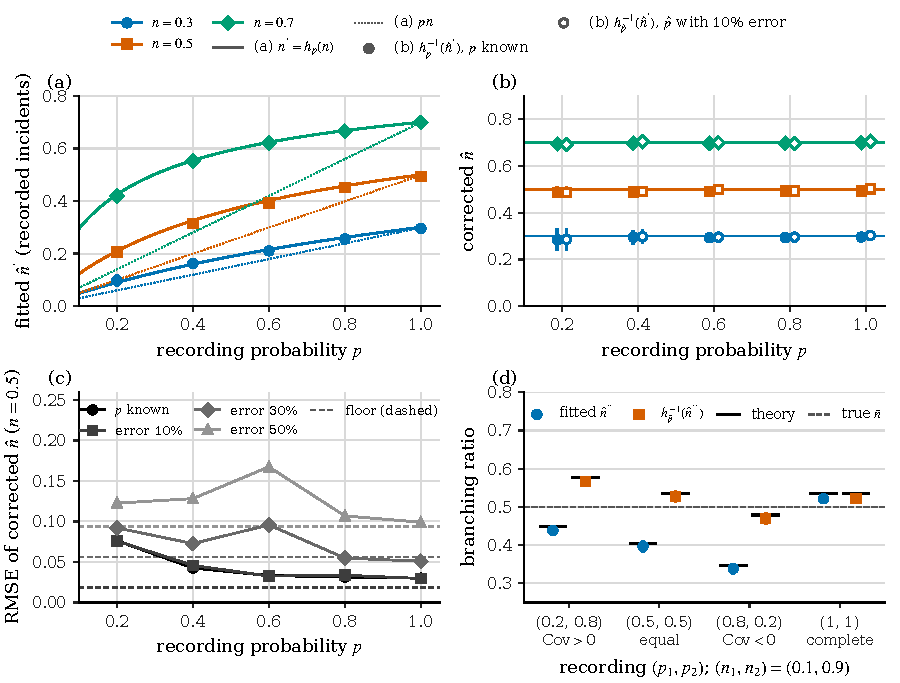
\includegraphics[width=6.0in]{figures/fig-sim-thinning.pdf}
\caption{E3, thinning (synthetic data; bars $\pm1.96$ MC SE). (a) Fitted branching ratio of
the recorded incidents against $p$, with $n'=h_p(n)$ (solid) and $pn$ (dotted); $R=40$. (b)
Corrected estimates with $p$ known (filled) or estimated with $10\%$ error (open); lines mark
the true $n$. (c) The variance floor at $n=0.5$: RMSE of the corrected estimate with $p$
known and with $10$, $30$ and $50\%$ error in $\hat p$, and the floor $r\,n(1-n)(2-n)/2$
(dashed); at $p=1$, $\hat p$ is clipped at $1$. (d) Heterogeneous recording of two marks
with $(n_1,n_2)=(0.1,0.9)$: fitted $\hat n''$ and the homogeneous correction against
\cref{prop:th-hetthin} (solid) and $\bar n=0.5$ (dashed); $R=30$.}
\label{fig:sim-thinning}
\end{figure}

\subsection{E4: the online-to-offline test and common shocks}\label{sec:sim-lrt}

Under $\alpha_{\mathrm{off},\mathrm{on}}=0$ the likelihood-ratio statistic should have the
chi-bar-square limit $\tfrac12\chi^2_0+\tfrac12\chi^2_1$ (\cref{prop:lrt}); an omitted
common shock that reaches online volume first should produce online-to-offline Granger
causality (\cref{rem:th-granger-caveats}(i)), and recording it should remove it
(\cref{cor:equiv-id}(i)). Two streams have
$\Amat=\bigl(\begin{smallmatrix}0.3&\alpha_{\mathrm{off},\mathrm{on}}\\0.2&0.4\end{smallmatrix}\bigr)$
and $T=600$; the shared decay stays identified under $H_0$ (\cref{rem:est-lrt}(i)). Common
shocks arrive at rate $0.05$ and reach the online stream within about half a day, the
offline stream over about four days. The test holds its size (\cref{tab:sim-e4e5}(a) and \cref{fig:sim-lrt}, both in
\cref{app:sim-e1e5}). Under $H_0$ ($R=160$) it rejects in $0.0875$ ($0.022$), $0.0625$
($0.019$) and $0.01875$ ($0.011$) of replicates at the $10$, $5$ and $1\%$ levels, and the
statistic is zero in $0.5625$ ($0.039$) of them; the naive $\chi^2_1$ reference rejects in
$0.025$ at $5\%$. The power is $0.617$, $0.983$ and $1.0$ for
$\alpha_{\mathrm{off},\mathrm{on}}=0.05$, $0.1$ and $0.2$ ($R=60$). With the common shocks
omitted the test rejects in all 60 replicates (mean estimate $0.072$), with no
online-to-offline excitation; with the calendar in the model it rejects in $0.083$
($0.036$), with mean estimate $0.010$. The Davies problem (\cref{sec:est-lrt}) was not
studied (its bootstrap needs about 600 EM fits per dataset); the block tests of the plan
need it, so it must pass the synthetic dry run (\cref{sec:plan-validation}, V4).

\subsection{E6: alerting and nowcasting}\label{sec:sim-alert}

\paragraph{Claim} Thresholding the predictive probability of a surge at $\pi^*$ minimises
the expected cost (\cref{thm:alert}(a)). If the predictive distribution is the conditional
law given the forecaster's information, the randomised PIT is uniform
(\cref{lem:fc-pit}(a)). Reporting delays bias the naive state downward, by the factor
$\E e^{-\beta d}$ under stationarity, and the delay-weighted state is unbiased
(\cref{prop:nowcast}).

\paragraph{Design} Two streams, offline (the target) and online, have
$\Amat=\bigl(\begin{smallmatrix}0.35&0.10\\0.25&0.45\end{smallmatrix}\bigr)$, and external
events arrive as a Poisson process at rate $1/30$ per day with log-normal sizes. Each of 12
replicates has a training period $[0,1000]$ and 150 weekly forecast windows. A surge is a window with at least $c=21$ offline
incidents, the 90th percentile in a separate pilot; the surge rate in the 1800 test windows
is $0.0967$ ($0.0070$). At each origin $t$ the predictive distribution of the offline count
is estimated from 2000 cluster continuations of the state at $t$ (\cref{lem:fc-future}),
with the true parameters or with EM estimates from the training period, in two versions.
One assumes \emph{no future events} after $t$. The other \emph{integrates} over them,
adding to each continuation the clusters of events drawn from the event process for
$(t,t+7]$ (true rate and size law, or those of the training calendar with fitted
loadings); this is the conditional law given the past, to which \cref{lem:fc-pit}(a)
applies (\cref{sec:fc-predictive}). The baselines are a moving-average Poisson forecast (mean of
the last four weekly counts) and climatology. Alerts use $c_{\mathrm{FA}}=1$ and
$c_{\mathrm{miss}}\in\{2,5,10\}$, so $\pi^*\in\{1/3,1/6,1/11\}$. Under delays
(offline only: zero with probability $0.3$, else exponential with mean three days), the
fitted forecast plugs the naive or the Horvitz--Thompson state (\cref{prop:nowcast}(b))
into the continuation. This plug-in is the shortcut that \cref{sec:fc-nowcast} warns is not
the Bayes rule for delayed data; \cref{alg:alert} itself was not run. Surges are defined by
the 90th rather than the plan's 95th percentile, and the baselines are not the plan's
background-only model and persistence rule (\cref{sec:plan-estimands}).

\paragraph{Decisions} The Hawkes rules have the lowest realised cost at every cost ratio
(\cref{tab:sim-e6}, \cref{fig:sim-alert}(a)), for example $0.285$ per window at
$c_{\mathrm{miss}}=5$ with true parameters against $0.451$ for the moving average and
$0.483$ for climatology, which is essentially the best constant rule. The comparison favours
the Hawkes model: the data are generated by it, and the baselines are simple ones, not the
plan's. Fitting the parameters costs almost nothing. Integrating over future events
changes the costs little (paired differences $-0.001$, $-0.002$ and $-0.014$, MC SEs
$0.002$, $0.007$ and $0.016$) but improves the Brier score from $0.0655$ to $0.0628$ (paired
MC SE $0.0006$). It raises the surge probability in every window, trading precision for
recall at $\pi^*=1/6$ ($0.503$ and $0.511$ against $0.614$ and $0.466$).

\paragraph{Calibration} Pooled over all windows, the forecast that integrates over future
events is calibrated (\cref{fig:sim-alert}(d)). With true parameters the PIT gives
$\chi^2=3.3$ on 9 degrees of freedom ($p=0.95$), and the mean forecast exceeds the outcome
by $0.07$ ($0.18$) incidents per window. With fitted parameters $\chi^2=17.1$ ($p=0.048$)
and the bias is $+0.38$ ($0.22$), because the event rate estimated from the training
calendar, $0.0353$ ($0.0018$) on average, exceeds $1/30$. The forecast that assumes no
future events is not calibrated: $\chi^2=175.3$, and it is too low by $1.91$ ($0.18$)
incidents per window with true parameters. That miscalibration comes from a misspecified
forecaster that leaves out the event process, not from the method. What no forecaster can
do is \emph{time} the events. In 108 of the 174 surge windows ($62\%$), an external event
arrives after the forecast origin. Conditionally on whether one arrives, even the
integrating forecast is not calibrated, and cannot be: its PIT values are too low in the
1424 windows without a new event and too high in the 376 with one, $36.4\%$ of them in the
top decile (\cref{fig:sim-alert}(e)). The limitation shows in recall: at $\pi^*=1/6$ the
integrating rule with true parameters detects $89\%$ of the surges in windows without a new
event but $28\%$ of those in windows with one. Alerts should be reissued as soon as a
salient event occurs.

\paragraph{Delays} The naive state is biased downward as \cref{prop:nowcast}(c) predicts:
with true parameters it averages $0.4752$ of the complete-data state, against
$\E e^{-\beta d}=0.475$, and never exceeds it; the Horvitz--Thompson state averages
$1.0033$ of it. In windows without a new event the no-future-event forecast from the naive
state is miscalibrated ($p=0.033$) and that from the nowcast is not ($p=0.435$). Neither
decisions nor pooled calibration show a benefit, however (\cref{tab:sim-e6},
\cref{fig:sim-alert}(b),(f)). With integration the three costs differ by at most $0.012$ at
each ratio, and at $c_{\mathrm{miss}}=5$ the naive state is even slightly cheaper than the
nowcast (paired difference $-0.008$, MC SE $0.003$): its forecasts are lower by $0.42$
incidents per window, which offsets the fitted forecaster's over-forecast. Here the delays
are short and the undelayed online stream carries much of the excitation. The study
confirms the correction of the state, not that the nowcast improves alert decisions.

\begin{table}[tbp]
\centering
\caption{E6, alerting (synthetic data; 12 replicates $\times$ 150 weekly windows). Realised
cost per window at $c_{\mathrm{miss}}/c_{\mathrm{FA}}=2$, $5$ and $10$ (MC SE
$0.008$--$0.06$); precision and recall at $\pi^*=1/6$; Brier score of the surge
probability; pooled PIT statistic $\chi^2_9$ ($5\%$ critical value $16.9$); mean forecast
minus outcome (Bias). ``No future events'': empty calendar after the forecast origin;
``integrating'': future events drawn from the event process. Delayed rows use fitted
parameters; climatology never alerts at $\pi^*=1/6$.}
\label{tab:sim-e6}
\footnotesize
\setlength{\tabcolsep}{4.5pt}
% Generated by code/make_figures.py from results/sim_results.json -- do not edit by hand.
% E6. Cost per window at c_miss/c_FA = 2, 5, 10; precision and recall at c_miss/c_FA = 5;
% Brier score of the surge probability; pooled PIT chi2 (9 df, 1800 windows); mean forecast minus outcome.
\begin{tabular}{@{}lrrrrrrrr@{}}
\toprule
 & \multicolumn{3}{c}{Cost per window} & & & & & \\
\cmidrule(lr){2-4}
Forecaster & 2 & 5 & 10 & Prec. & Recall & Brier & PIT $\chi^2_9$ & Bias \\
\midrule
\multicolumn{9}{@{}l}{\emph{Complete data}} \\
\quad Hawkes, true par., no future events & 0.137 & 0.287 & 0.526 & 0.614 & 0.466 & 0.0655 & 175.3 & $-$1.91 \\
\quad Hawkes, true par., integrating & 0.136 & 0.285 & 0.512 & 0.503 & 0.511 & 0.0628 & 3.3 & $+$0.07 \\
\quad Hawkes, fitted, no future events & 0.137 & 0.287 & 0.534 & 0.594 & 0.471 & 0.0654 & 169.8 & $-$1.75 \\
\quad Hawkes, fitted, integrating & 0.134 & 0.289 & 0.514 & 0.484 & 0.511 & 0.0629 & 17.1 & $+$0.38 \\
\quad Moving-average Poisson & 0.221 & 0.451 & 0.792 & 0.216 & 0.247 & 0.1141 & 1994.3 & $+$0.06 \\
\quad Climatology & 0.193 & 0.483 & 0.898 & --- & 0.000 & 0.0880 & 26.5 & $+$0.94 \\
\addlinespace
\multicolumn{9}{@{}l}{\emph{Reporting delays}} \\
\quad Fitted, naive state, no future events & 0.138 & 0.304 & 0.518 & 0.629 & 0.420 & 0.0668 & 247.8 & $-$2.18 \\
\quad Fitted, HT nowcast, no future events & 0.135 & 0.297 & 0.523 & 0.572 & 0.454 & 0.0654 & 190.5 & $-$1.75 \\
\quad Fitted, naive state, integrating & 0.137 & 0.279 & 0.502 & 0.550 & 0.506 & 0.0633 & 6.8 & $-$0.05 \\
\quad Fitted, HT nowcast, integrating & 0.135 & 0.287 & 0.510 & 0.481 & 0.517 & 0.0630 & 13.3 & $+$0.37 \\
\quad Moving-average Poisson, available counts & 0.226 & 0.478 & 0.848 & 0.177 & 0.161 & 0.1130 & 1879.8 & $-$0.65 \\
\bottomrule
\end{tabular}

\end{table}

\begin{figure}[t]
\centering
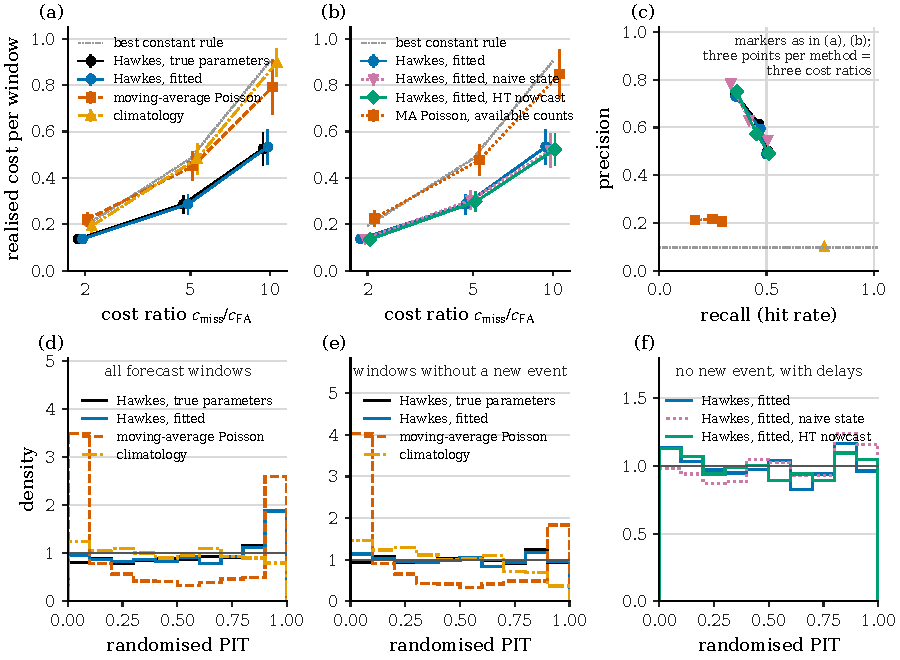
\includegraphics[width=6.0in]{figures/fig-sim-alert.pdf}
\caption{E6, alerting and nowcasting (synthetic data; 12 replicates $\times$ 150 weekly
windows; bars $\pm1.96$ MC SE). Hawkes forecasts with true or fitted parameters, assuming no
future events (dashed, open markers) or integrating over them (solid, filled). (a) Realised
cost per window against the cost ratio; dotted: best constant rule. (b) The same under
reporting delays (fitted, integrating). (c) Precision against recall at the three
thresholds; dotted: surge rate. (d) PIT histograms, all windows. (e) PIT of the integrating
forecast with true parameters, for windows in which an external event arrives after the
origin and for the others. (f) PIT under delays, all windows.}
\label{fig:sim-alert}
\end{figure}

\subsection{What the study does and does not show}\label{sec:sim-limits}

Under the model the tools work as the theory says: EM recovers the branching matrix and
the surge decomposition with close to nominal coverage, the boundary test holds its size,
and the dark-figure correction restores coverage except when excitation is weak and
recording poor, with a floor of about $0.04$--$0.09$ set by a $30$--$50\%$ error in $p$. The
traps are real: a constant background finds contagion where there is none (for rare large
shocks $0.06$--$0.07$ below $n^*$ even with $T=10{,}000$); smoothing does not remove the
artefact of fast shocks, while the shock times largely do, where tested; and an omitted
common shock creates an online-to-offline effect. On Hawkes-generated data a plug-in Hawkes
alert rule beats two simple baselines that are not the plan's. Forecasts that integrate
over future events are calibrated when pooled; no forecaster can time the events, and that
limits recall.

The study has clear limits. Each experiment uses a few parameter points, at most three
streams, exponential kernels and, apart from E2, constant backgrounds; there are no
near-critical systems and no misspecified kernels. The replicate numbers resolve
differences of a few hundredths in branching ratios and about $0.01$--$0.04$ in costs, not
smaller ones. Not evaluated were the Davies sup-test and its bootstraps, Bayesian
estimation and shrinkage, the INAR approximation, nonparametric kernels, the time-rescaling
check, placebo calibration and the imputation algorithm (\cref{alg:alert}); the delay
correction was evaluated only as a plug-in state. Nor did we test whether a flexible
background absorbs genuine contagion, long windows for slow switching, or the selection
rules of the analysis plan. These checks belong to the synthetic dry run of the plan
(\cref{sec:plan-validation}, V4).
